\chapter{半导体中的电子状态}

半导体具有许多独特的物理性质,这与半导体中电子的状态及其运动特点有密切关系。为了研究半导体的这些物理性质,本章将简要介绍半导体单晶材料中的电子状态及其运动规律。

半导体单晶材料和其他固态晶体一样,是由大量原子周期性重复排列而成,但这是一个非常复杂的多体问题,直接求解其薛定谔方程是无法做到的,只能采取近似的方法,称为\uwave{单电子近似}。所谓单电子近似,即假设每个电子是在周期性排列且固定不动的原子核势场及其他电子的平均势场中运动,并且势场是与晶格同周期的周期性势场。这种通过单电子近似法研究晶体中电子状态的理论,称为\uwave{能带理论}(Band Theorey)。能带的概念是半导体物理的核心。

\section{半导体的晶体结构}

\subsection{金刚石结构}
重要的半导体材料,包括硅\xce{Si}、锗\xce{Ge}等在化学元素周期表中都属于第\Romnum{4}族元素,原子的最外层都具有$4$个价电子。硅原子和锗原子组成晶体时依靠的是共价键的结合,它们的晶格结构与碳原子构成的金刚石结构一致,关于金刚石结构,我们在固体物理中已经有了比较清楚的认识,简而言之,每个原子的四个最近邻原子以正四面体的方式分布,即配位数为$4$。

金刚石结构可用\xref{fig:金刚石结构的俯视投影}的俯视投影表示,对比固体物理中的立体图很容易理解
\begin{Figure}[金刚石结构的俯视投影]
    \includegraphics[scale=0.55]{build/Chapter01A_01.fig.pdf}
\end{Figure}
\xref{fig:金刚石结构的俯视投影}中,虚线是晶胞边界,数字是该原子距晶胞顶面的距离(几倍晶格常数)。

金刚石结构的共价键晶体中,每个原子的$4$个共价键是完全等价的,这是怎么实现的呢?实际上,它们是由$1$个s态和$3$个p态线性组合而成的$4$个sp$^{3}$杂化轨道,键角为$109^\circ 28'$。

金刚石的每个晶胞中,共有$8$个原子(顶点$1$个、侧面$3$个、内部$4$个),实验测得
\begin{Table}[硅和锗的晶体参数]{lrrrr}
    <元素&晶格常数(\si{nm})&单位体积原子(\si{cm^3})&原子最短间距(\si{nm})&原子的共价半径(\si{nm})\\>
    硅&$0.543102$&$5.00\times 10^{22}$&$0.235$&$0.117$
    \\
    锗&$0.565791$&$4.42\times 10^{22}$&$0.245$&$0.122$\\
\end{Table}
由晶格常数$a$可知晶格体积为$a^3$,单位体积的晶格数即$1/a^3$,单位体积的原子数即$8/a^3$,考虑导金刚石的每个晶胞具有$8$个原子(特别注意单位换算,上述单位体积是单位立方厘米)。

\subsection{闪锌矿和纤锌矿结构}
实际上,除了硅和锗这样的半导体,许多\Romnum{3}--\Romnum{5}族化合物和\Romnum{2}--\Romnum{6}族化合物都是半导体。

化合物半导体通常有两种主要构型
\begin{itemize}
    \item 闪锌矿结构,主要出现在化合键中共价键成分比较高的情况。
    \item 纤锌矿结构,主要出现在化合键中离子键成分比较高的情况。
\end{itemize}
化合物中,\Romnum{3}--\Romnum{5}族呈闪锌矿结构,\Romnum{2}--\Romnum{6}族则能以闪锌矿和纤锌矿两种方式结晶。

\begin{Figure}[纤锌矿结构]
    \vspace{-0.5cm}
    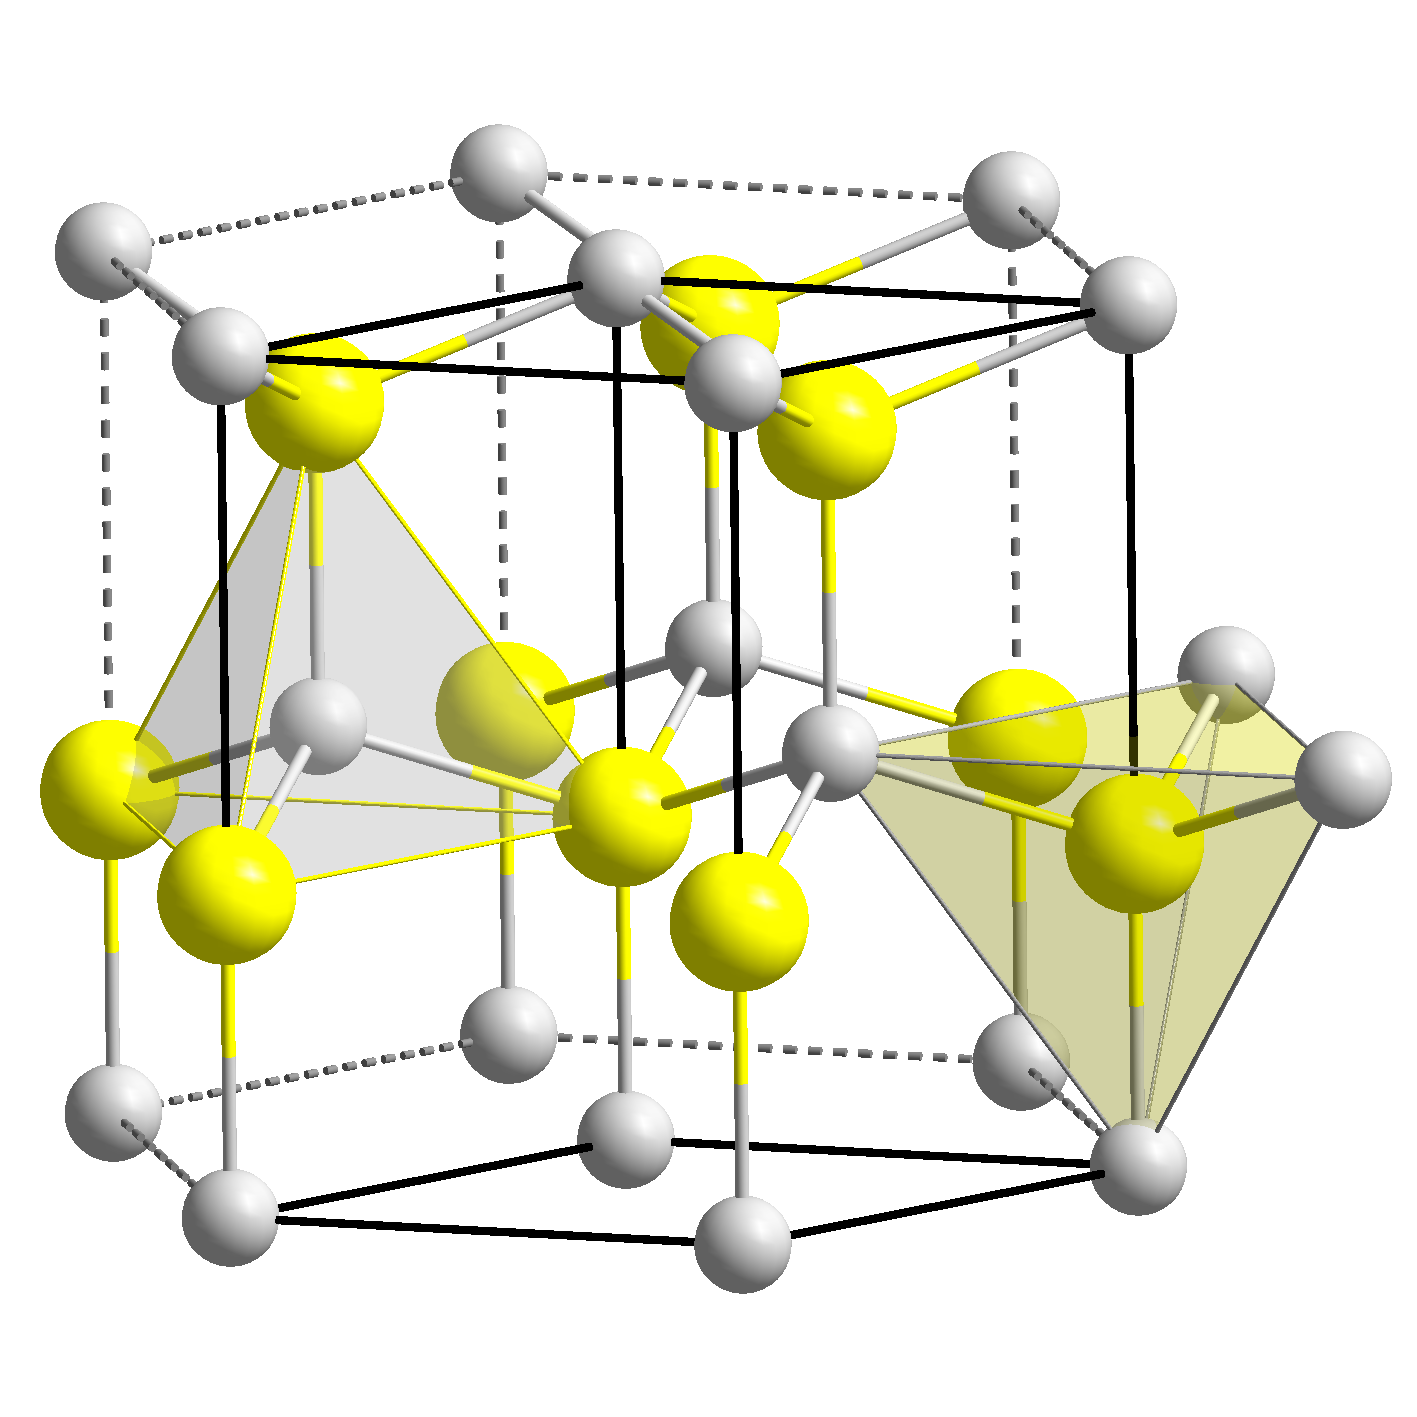
\includegraphics[width=6cm]{image/Wurtzite_polyhedra.png}
    \vspace{-0.5cm}
\end{Figure}

闪锌矿结构是我们在固体物理中比较熟悉的,它与金刚石结构非常相似,但不同的是,闪锌矿结构中$A,B$两类原子分别由化合物中的两种不同原子构成。纤锌矿结构则是一种新的晶体结构,如\xref{fig:纤锌矿结构}所示\cite{W1},纤锌矿结构和闪锌矿结构一样,两类原子都位于对方构成的正四面体的中心,但是,纤锌矿具有六方对称性,具体的说,两类原子自身先构成六角点阵(这里六角点阵上下底面的中间还有三个格点),随后,两类原子的点阵上下将错开略小于$c/2$的距离,这里$c$是六角点阵的高,而准确的错开距离,即略小于$c/2$多少由构成正四面体的要求确定。
\section{半导体中的能带结构}

\subsection{能级分裂与能带}
原子中的电子在原子核的势场和其他电子的作用下,它们分列在不同的能级桑,形成电子壳层,分别用1s, 1s, 2p, 3s, 3p, 3d等符号表示,每一电子壳层对应与一个确定的能级。原子相互接近形成晶体时,不同原子的电子壳层之间就有了一定程度的交叠,此时,电子不再局限于某一个原子上,而是可以由一个原子转移到相邻的原子上去,因而,电子将可以在整个晶体中运动,称为电子的共有化运动,但需要注意的是,电子只能在相同能级的壳层之间转移
\begin{itemize}
    \item 内层壳层的交叠较弱,因此内层壳层对应的共有化运动较弱。
    \item 外层壳层的交叠较强,因此外层壳层对应的共有化运动较强。
\end{itemize}
原子构成晶体后,电子做共有化运动时能量又是怎么样的呢?如\xref{fig:能级分裂与能带}所示,设想由$N$个原子构成的晶体(通常$N$是很大的数值),假设$N$个原子最初相距很远,尚未结合成晶体时,而此时,每个原子都可以视为孤立原子,每个原子的电子都具有相同的1s, 2s, 2p等能级,或者说,此时电子在1s, 2s, 2p上是$N$重简并的\footnote{所谓简并,就是指一系列特征函数具有相同的特征值,更具体的说,就是指一系列不同的电子波函数具有相同的能量。},而当$N$个原子逐渐靠近结合为晶体时,我们知道,电子作为一种费米子需要遵循泡利不相容准则,因此,电子的$N$重简并之间将产生逐渐增大的排斥,从而促使原先的每个能级分裂为$N$个彼此相距很近的能级,由于原子数$N$的值非常大,这$N$个能级组成一个准连续的\uwave{能带}(Energy Band)。即,原子在孤立状态下电子能量只能取一系列的分立值,原子在晶体状态下电子能量就可以在一系列的分立的区间中取值
\begin{itemize}
    \item 我们将晶体状态下,电子能量允许取值的那些区间,称为\uwave{允带}(Permitted Band)。
    \item 我们将晶体状态下,电子能量不能取值的那些区间,称为\uwave{禁带}(Forbidden Band)。
\end{itemize}
\begin{Figure}[能级分裂与能带]
    \includegraphics[scale=0.68]{build/Chapter01B_01.fig.pdf}
\end{Figure}
很明显,允带和禁带是相互交错的,它们互为彼此的空隙。

需要说明的是,如果原先的能级本身就具有简并,例如2p三重简并了2p$_x$,2p$_y$,2p$_z$三个不同取向的轨道,那么这种简并会在能级分裂时一并被释放,例如2p分裂后将产生$3N$个能级。

除此之外,能级分裂的程度并不是相同的,如\xref{fig:能级分裂与能带}
\begin{itemize}
    \item 内层电子原先处于低能级,共有化运动弱,其能级分裂很小,能带很窄。
    \item 外层电子原先处于高能级,共有化运动强,其能级分裂很大,能带很宽。
\end{itemize}

但是,由于杂化作用的影响,包括金刚石结构在内的硅和锗的能带与能级其实并不是一一对应的,如\xref{fig:能级分裂与能带}所示,首先2s的一个轨道与2p的三个轨道将杂化为四个2sp$^3$的轨道,每个轨道上各有一个电子,故$N$个原子共有$4N$个电子。然而,与我们的预期有些不符
\begin{itemize}
    \item 四重简并的2sp$^3$的轨道并未分裂为$1$个具有$4N$个能级的能带。
    \item 四重简并的2sp$^3$的轨道将会分裂为$2$个具有$2N$个能级的能带。
\end{itemize}
在这两个能带中,有一个能带能量低于2sp$^3$能级,有一个能带能量高于2sp$^3$能级,两者中的轨道分别称为\uwave{成键轨道}(Bonding Orbit)和\uwave{反键轨道}(Antibonding Orbit),显然$4N$个电子将完全填充在能量较低的$2N$个成键轨道,而能量较高的$2N$个反键轨道上则没有任何电子填充,将两者构成的能带,分别称为\uwave{价带}(Valence Band)和\uwave{导带}(Conduction band)。\cite{W2}

\begin{Figure}[能级分裂与能带]
    \includegraphics[scale=0.68]{build/Chapter01B_02.fig.pdf}
\end{Figure}

简而言之,价带和导带是允带的两个细分概念\footnote{允带给出只是电子允许存在的能量,但是这些能量未必真的填充有电子。},\empx{价带中填满了电子},\empx{导带中没有电子}。

因此,价带也称为\uwave{满带}(Filled Band),导带也称为\uwave{空带}(Empty Band)。

\subsection{能带的定量分析}
在\xref{subsec:能级分裂与能带}中,我们定性的对比了晶体中的电子和孤立原子的电子的差异,阐述了能级是如何分裂并演化为能带的,而在这一小节,我们将定量研究晶体中的电子和自由电子的关系。

实际上,从定态薛定谔方程的角度看
\begin{eqnarray}
    -\frac{\hbar^2}{2m_e}\dv[2]{\psi}{x}+V(x)\psi=E\psi
\end{eqnarray}
自由电子即势能$V(x)=0$恒为零,晶体中的电子即势能$V(x)=V(x+a)$具有晶格周期性。

自由电子的波函数就是普通的平面波
\begin{Equation}
    \psi_k(x)=A\e^{\i kx}
\end{Equation}
自由电子的能量本征值(色散关系)满足抛物线关系
\begin{Equation}
    E(k)=\frac{\hbar^2k^2}{2m_e^2}
\end{Equation}
自由电子的波矢$k$可以连续取值,因此,自由电子的能量是连续能谱,任意取值都是允许的。


布洛赫曾经证明过,周期性势场$V(x)=V(x+a)$中的波函数必具有以下形式
\begin{BoxTheorem}[布洛赫定理]
    若势场$V(x)$具有周期性$V(x)=V(x+a)$,则其波函数一定有以下形式
    \begin{Equation}
        \psi_k(x)=A_k(x)\e^{\i kx}\qquad A_k(x)=A_k(x+a)
    \end{Equation}
    该结论称为\uwave{布洛赫定理}(Bloch's Theorem)。
\end{BoxTheorem}
布洛赫定理告诉我们,晶体周期性势场中的电子波函数具有$\psi_k(x)=A_k(x)\e^{\i kx}$的形式,通过和自由电子波函数$\psi_k(x)=A\e^{\i kx}$的对比,我们可以看出,\empx{晶体中的电子是以一个被周期性调幅的平面波在晶体中传播},振幅$A_k(x)$随$x$依照晶格周期$a$作周期性变化。除此之外,根据波函数的意义,在空间某点找到电子的概率密度与$|\psi|^2$成正比,因此,自由电子在空间格点处的概率密度$|\psi|^2=A^2$处处相同,晶体中的电子的概率密度$|\psi|^2=|A_kA_K^{*}|$则是周期性的。

现在的问题是,我们已经知道晶体中电子的波函数了,那么晶体中电子的能量本征值$E(k)$与波矢$k$的关系是什么呢?这是比较复杂的,我们直接在\xref{tab:能带结构的三种图示}中给出图像,我们注意到
\begin{enumerate}
    \item 重复区表示法是最完整的图像,我们看到,晶体中的电子能量$E(k)$与波矢$k$间的关系有若干组$E_1(k), E_2(k), E_3(k), \cdots$,这些色散关系均具有周期性,并且,这些色散关系两两之间不重叠,而是有一定间隙,这些间隙就是禁带,而每个$E(k)$就给出了一个允带。
    \item 扩展区表示法是指,将各组$E(k)$分别对应到各个布里渊区,我们以$E_n(k)$对应第$n$布里渊区,这种表示法的好处是,我们可以看到,晶体中电子的$E(k)$关系的整体趋势上,其实很接近自由粒子$E(k)$的抛物线关系,但是,能量在布里渊区的边界$\pm n\pi/a$处会出现不连续,因此我们常说,\empx{每个布里渊区对应一个允带},\empx{禁带出现在布里渊区的边界}。\footnote{尽管能带图只是关于能量的一维关系,与波矢和布里渊区并没有什么关系。}
    \item 约化区表示法是指,将各组$E(k)$利用周期性简约在第一布里渊区$[-\pi/a,+\pi/a]$。
\end{enumerate}
晶体中的原子数$N$总是有限的,考虑周期性边界条件,波矢$k$只能分立取值
\begin{Equation}
    k=\frac{2\pi n}{Na}\qquad n=0,\pm 1,\pm 2,\cdots
\end{Equation}
因此在第一布里渊区中$k$只有$N$个分立的取值,但由于$N$很大,可以认为是准连续的。
\begin{TableLong}[能带结构的三种图示]{|c|}
<>()
< >( )
    \xcell<c>[1.5ex][0.0ex]{\includegraphics[scale=0.95]{build/Chapter01B_03.fig.pdf}}\\*
    \xgp[0ex][3ex]{重复区表示法}\\ \hlinemid
    \xcell<c>[1.5ex][0.0ex]{\includegraphics[scale=0.95]{build/Chapter01B_04.fig.pdf}}\\*
    \xgp[0ex][3ex]{扩展区表示法}\\ \hlinemid
    \xcell<c>[1.5ex][0.0ex]{\includegraphics[scale=0.95]{build/Chapter01B_05.fig.pdf}}\\*
    \xgp[0ex][3ex]{约化区表示法}\\ \hlinemid
\end{TableLong}
\section{半导体中的载流子}

\subsection{有效质量的引入}
晶体中电子的能量形成能带,而$E(k)$和$k$的关系如\xref{tab:能带结构的三种图示}所示,但事实是,我们仅仅是半定量的确定了$E(k)$是$k$的周期函数,仍然没有得出$E(k)$的具体形式,这确实是很繁琐的。

不过,对于半导体而言,由于起作用的常常是接近价带顶部或导带底部处的电子,因此,只要掌握其价带底部和导带顶部,也就是能带极值处$E(k)$与$k$的关系式就可以了,而这就给我们的近似计算提供了可能。近似技巧是应用泰勒级数,假设能带极值位于波矢$k=0$处,由于能带底部附近的$k$值必然很小,因此可以将$E(k)$在$k=0$处泰勒展开,并仅取至二次项,得到\setpeq{有效质量的引入}
\begin{Equation}&[1]
    E(k)=E(0)+\eval{\dv{E}{k}}_{k=0}k+\frac{1}{2}\eval{\dv[2]{E}{k}}_{k=0}k^2
\end{Equation}
这里,由于在能带极值处一阶导数为零,即$(\dv*{E}{k})|_{k=0}=0$,故
\begin{Equation}&[2]
    E(k)-E(0)=\frac{1}{2}\eval{\dv[2]{E}{k}}_{k=0}k^2
\end{Equation}
这里$E(0)$是该能带底部的能量,而对于给定半导体,这里$(\dv*[2]{E}{k})$应该是一个定值。

基于此,我们可以定义一个代换变量(我们马上会看到它为什么称为“质量”)
\begin{BoxDefinition}[有效质量]
    定义半导体中的电子,在能带极值处的\uwave{有效质量}(Effective Mass)$\mne$为
    \begin{Equation}
        \frac{1}{\mne}=\frac{1}{\hbar^2}\eval{\dv[2]{E}{k}}_{k=0}
    \end{Equation}
\end{BoxDefinition}
运用有效质量的概念,\xrefpeq[有效质量的引入]{2}就可以改写为
\begin{Equation}
    E(k)-E(0)=\frac{\hbar^2k^2}{2\mne}
\end{Equation}
这和先前自由电子的能量表达式非常接近
\begin{Equation}
    E(k)=\frac{\hbar^2k^2}{2m_e}
\end{Equation}
唯一的差异是,电子的质量$m_e$被替换了能带极值处电子的有效质量$\mne$,换言之,\empx{半导体中位于能带极值处的电子的行为,可以用特定质量的自由电子等效}。我们知道,半导体中的电子会受到大量原子核和大量其他电子的群体作用,而现在,我们将这种群体作用的结果用一个特定质量简单的自由电子来代替。从这样的观点看,半导体中的电子在应用上述能带极值处的等效后,实际上,是一种\uwave{准粒子}(Quasiparticles)或\uwave{集体激发}(Collective Excitations)。\cite{W3}

有效质量,依据上述讨论,其实也就是半导体中电子对应的“准粒子”的“准质量”了,简洁起见,我们后面不再区分“半导体中的电子”和“半导体中的电子对应的准粒子”的提法。

有效质量$\mne$可以是正的,也可以是负的
\begin{itemize}
    \item 价带顶部处$E(0)>E(k)$,因此,价带顶部的有效质量$\mne<0$。
    \item 导带底部处$E(0)<E(k)$,因此,导带底部的有效质量$\mne>0$。
\end{itemize}

接下来,我们来看有效质量是如何与我们认知中的质量相一致的。

\subsection{半导体中电子的速度}\setpeq{半导体中电子的速度}
根据量子力学的概念,电子的运动速度相当于其波包的群速
\begin{Equation}&[1]
    v=\dv{\omega}{k}
\end{Equation}
在该式中,代入德布罗意关系$E=\hbar\omega$
\begin{Equation}&[2]
    v=\frac{1}{\hbar}\dv{E}{k}
\end{Equation}
在上式中将能量$E$用有效质量表示
\begin{Equation}&[3]
    v=\frac{1}{\hbar}\dv{k}\qty(\frac{\hbar^2k^2}{2\mne}+E_0)=\frac{\hbar k}{\mne}    
\end{Equation}
由此,半导体中电子的速度就可以用其有效质量表示了
\begin{BoxFormula}[半导体中电子的速度]
    半导体中,电子的速度可以用有效质量表示为
    \begin{Equation}
        v=\frac{\hbar k}{\mne}
    \end{Equation}
\end{BoxFormula}

\subsection{半导体中电子的加速度}\setpeq{半导体中电子的加速度}
实际中,许多半导体器件都在一定的外加电压下工作,这样一来,半导体内部就产生了外加电场,这种情况下,电子还会受到外加电场力的作用,那此时,电子将会以何种规律运动?

我们要回答的其实就是,如果电子受力为$f$,那么电子的加速度是多少?

计算外力$f$对电子做的功
\begin{Equation}&[1]
    \dd{E}=f\dd{s}=fv\dd{t}
\end{Equation}
将\xrefpeq[半导体中电子的速度]{2}中$v=(\dv*{E}{k})/\hbar$代入上式
\begin{Equation}&[2]
    \dd{E}=\frac{f}{\hbar}\dv{E}{k}\dd{t}
\end{Equation}
但很显然的是
\begin{Equation}&[3]
    \dd{E}=\dv{E}{k}\dd{k}
\end{Equation}
这样,对比一下\xrefpeq{2}和\xrefpeq{3}
\begin{Equation}&[4]
    \frac{f}{\hbar}\dd{t}=\dd{k}
\end{Equation}
这样就可以确定$f$
\begin{Equation}&[5]
    f=\hbar\dv{k}{t}
\end{Equation}
这就表明,\empx{电子波矢的变化率正比于外力},而根据\fancyref{fml:半导体中电子的速度},既然此处电子的波矢在变化,那么电子的速度也必然在变化,这就意味着,电子将具有加速度。

在加速度定义的基础上应用\xrefpeq[半导体中电子的速度]{2},即$v=(\dv*{E}{k})/\hbar$
\begin{Equation}&[6]
    a=\dv{v}{t}=\frac{1}{\hbar}\dv{t}\qty(\dv{E}{k})=\frac{1}{\hbar}\dv[2]{E}{k}\dv{k}{t}
\end{Equation}
在上式中代入\xrefpeq{5}
\begin{Equation}
    a=\frac{f}{\hbar^2}\dv[2]{E}{k}
\end{Equation}
根据\fancyref{def:有效质量},即$(1/\mne)=(\dv*[2]{E}{k})/\hbar^2$
\begin{Equation}
    a=\frac{f}{\mne}
\end{Equation}

这就表明,电子所受外力与加速度的关系,在使用有效质量时符合牛顿第二定律。
\begin{BoxFormula}[半导体中电子的加速度]
    半导体中,电子的加速度和所受外力间满足以下关系
    \begin{Equation}
        a=\frac{f}{\mne}
    \end{Equation}
\end{BoxFormula}

\subsection{空穴的进一步讨论}
在\xref{subsec:能带与固体导电性}中曾提到,导带中是电子导电,价带中是空穴导电。实际上,空穴也可以视为一种准粒子,因为,空穴的实质是电子群体运动导致的在能带上移动的空量子态。既然空穴是准粒子,它也可以定义有效质量的概念,那么,空穴的有效质量和电子的有效质量有何种关系?

\begin{BoxFormula}[空穴和电子的有效质量的关系]
    空穴的效质量$\mpe$总是相应电子有效质量$\mne$的负值
    \begin{Equation}
        \mpe=-\mne
    \end{Equation}
\end{BoxFormula}
在这里,让我们来总结一下
\begin{itemize}
    \item 价带中空穴导电,空穴带正电,空穴质量$\mpe$是价带顶电子有效质量的负值。
    \item 导带中电子导电,电子带负电,电子质量$\mne$是导带底电子有效质量的正值。
\end{itemize}
价带顶电子有效质量为负,导带底电子有效质量为正,因此,\empx{电子和空穴的质量均为正}。






